%%%%%%%% ICML 2021 EXAMPLE LATEX SUBMISSION FILE %%%%%%%%%%%%%%%%%

\documentclass{article}

% Recommended, but optional, packages for figures and better typesetting:
\usepackage{microtype}
\usepackage{graphicx}
\usepackage{subfigure}
\usepackage{booktabs} % for professional tables

% hyperref makes hyperlinks in the resulting PDF.
% If your build breaks (sometimes temporarily if a hyperlink spans a page)
% please comment out the following usepackage line and replace
% \usepackage{icml2021} with \usepackage[nohyperref]{icml2021} above.
\usepackage{hyperref}

% Attempt to make hyperref and algorithmic work together better:
\newcommand{\theHalgorithm}{\arabic{algorithm}}

% Use the following line for the initial blind version submitted for review:
\usepackage{icml2021}

% If accepted, instead use the following line for the camera-ready submission:
%\usepackage[accepted]{icml2021}

% The \icmltitle you define below is probably too long as a header.
% Therefore, a short form for the running title is supplied here:
\icmltitlerunning{Diagnosing Brain Disorders with Deep Anomaly Detection}

\begin{document}
	
	\twocolumn[
	\icmltitle{Diagnosing Brain Disorders with Deep Anomaly Detection}
	
	% It is OKAY to include author information, even for blind
	% submissions: the style file will automatically remove it for you
	% unless you've provided the [accepted] option to the icml2021
	% package.
	
	% List of affiliations: The first argument should be a (short)
	% identifier you will use later to specify author affiliations
	% Academic affiliations should list Department, University, City, Region, Country
	% Industry affiliations should list Company, City, Region, Country
	
	% You can specify symbols, otherwise they are numbered in order.
	% Ideally, you should not use this facility. Affiliations will be numbered
	% in order of appearance and this is the preferred way.
	\icmlsetsymbol{equal}{*}
	
	\begin{icmlauthorlist}
		\icmlauthor{Amr Farahat}{equal,FIAS}
		\icmlauthor{Diyuan Lu}{equal,FIAS, CePTER}
		\icmlauthor{Sebastian Bauer}{Klinic, CePTER}
		\icmlauthor{Valentin Neubert}{Rostock}
		\icmlauthor{Lara Sophie Costard}{Royal}
		\icmlauthor{Felix Rosenow}{Klinic, CePTER}
		\icmlauthor{Jochen Triesch}{FIAS, CePTER}
	\end{icmlauthorlist}
	
	\icmlaffiliation{FIAS}{Frankfurt Institute for Advanced Studies, Germany}
	\icmlaffiliation{Klinic}{Epilepsy Center Frankfurt Rhein-Main, University Hospital Goethe-University, Germany}
	\icmlaffiliation{CePTER}{Center for Personalized Translational Epilepsy Research (CePTER), Frankfurt am Main, Germany}
	\icmlaffiliation{Rostock}{Oscar Langendorff Institute of Physiology, Rostock University Medical Center, Rostock, Germany}
	\icmlaffiliation{Royal}{Tissue Engineering Research Group, Royal College of Surgeons Ireland, Dublin, Ireland}
	
	
	\icmlcorrespondingauthor{Jochen Triesch}{triesch@fias.uni-frankfurt.de}
	
	% You may provide any keywords that you
	% find helpful for describing your paper; these are used to populate
	% the "keywords" metadata in the PDF but will not be shown in the document
	\icmlkeywords{Early diagnosis, Epileptogenesis, time series anomaly detection, adversarial VAE}
	
	\vskip 0.3in
	]
	
	% this must go after the closing bracket ] following \twocolumn[ ...
	
	% This command actually creates the footnote in the first column
	% listing the affiliations and the copyright notice.
	% The command takes one argument, which is text to display at the start of the footnote.
	% The \icmlEqualContribution command is standard text for equal contribution.
	% Remove it (just {}) if you do not need this facility.
	
	%\printAffiliationsAndNotice{}  % leave blank if no need to mention equal contribution
	\printAffiliationsAndNotice{\icmlEqualContribution} % otherwise use the standard text.
	
	\begin{abstract}
		We consider a generalizable framework for diagnosing brain disorders from EEG recordings, in which a generative model is trained to detect any systematic deviations from the normal EEG signal. Mesial Temporal Lobe Epilepsy (mTLE) is an acquired disorder that usually follows brain injury by a latent period, in which the epileptogenesis (EPG) process occurs. Early diagnosis of latent EPG in epilepsy development prior to the first spontaneous seizure is crucial for the prognosis, however challenging, due to lack of reliable bio-markers and hard-to-obtain data annotations. Formulated as a binary classification problem, supervised deep learning methods have proven promising in differentiating between EEG data recorded before vs. after the induced brain injury by perforant pathway stimulation in a mTLE rodent model. For sake of generalizability to other brain disorders, we propose to reformulate the problem as an unsupervised anomaly detection, in which we train an adversarial autoencoder (AAE) to learn to encode normal EEG data into a low-dimensional latent space with an imposed prior distribution. The trained model is then used to scan the entire latent period to identify  anomalous epileptogenic data represented by two metrics: high reconstruction errors and large distance of the encoded embedding from the latent space prior distribution. Preliminary results show that reconstruction errors increase as a function of time after the induced brain injury until the occurrence of the first seizure which hints at a gradual epileptogenic process that changes the features of the EEG signals. Moreover, combining evidence from both metrics leads to more robust and generalizable results across different rats. In conclusion, we demonstrate that unsupervised learning methods can be used to automatically detect systematic drifts in brain activity patterns occurring over long time periods. This could facilitate rapid diagnosis of brain diseases and open the door for early interventions.
	\end{abstract}
	
	% TODO: what are the anomaly waveforms? Are they indicative?
	\section{Introduction}
	%XX is an important problem in ML and healthcare.  (Make
	%sure that the clinicians can see the relevance! \emph{Unclear clinical
	%	relevance is a major reason that otherwise strong-looking papers are
	%	scored low/rejected.})
	%
	%Addressing this problem is challenging because XX.  (Make sure that
	%you connect to the ML here.)  
	%
	%Others have tried, but XX remains tough.  (Acknowledge related work.)
	%
	%In this work, we...
	%
	%As you write, keep in mind that MLHC papers are meant to be read by
	%computer scientists and clinicians.  In the later sections, you might
	%have to use some medical terminology that a computer scientist may not
	%be familiar with, and you might have to use some math that a clinician
	%might not be familiar with.  That's okay, as long as you've done your
	%best to make sure that the core ideas can be understood by an informed
	%reader in either community.
	% Eearly diagnosis of epilepsy, mTLE
	Early diagnosis of epilepsy before the first spontaneous seizure is essential to open the door to future care and timely treatment \cite{moshe2015epilepsy}. Since over 30\% of the epilepsy patients will become pharmaco-resistant and suffer from recurring seizures for the rest of their lives \citep{kwan2000early}. Hence, it is of great importance to identify patients with a high risk before epilepsy is fully established. There often is a latent latent period between the brain injury and the onset of the first spontaneous seizure (FSS). The term epileptogenesis (EPG) is the process where the healthy brain transformed to epileptic brain, capable of generating spontaneous recurring seizures \cite{loscher2019holy, pitkanen2014past}.  Over 30\% of the patients will be pharmaco-resistant and continue to suffer from recurring seizures despite intake of medications \citep{kwan2000early}. The more seizure episodes have occurred before the first clinical visit, the less effective of the treatment will be \citep{kwan2000early}. Hence, identifying the presence of EPG before the epilepsy is fully established would be of great importance. However, the process of EPG is still not fully understood \citep{pitkanen2016advances}. The precise time of onset of the brain being epileptogenic is untraceable.
	
	Recently advances in machine learning (ML) and deep learning (DL) offers promising directions. Applying DL-based method to epilepsy research have delivered encouraging results. \cite{lu2020towards}
	
	Here, we proposed a more general framework for detecting brain disorders in a complete unsupervised fashion based on the idea of anomaly detection.
	
	% conventional anomaly detection
	Anomaly detection (AD) is one class of problems applying supervised learning, semi-supervised, or unsupervised method to detect out of distribution samples given the availability of sample labels \cite{NEURIPS2019_805163a0}.
	
	% classic anomaly detection
	downside is to face the large and rapidly growing data size.
	How to leverage deep learning for anomaly detection and apply to medical diagnosis is not clear.
	
	% the difference in medical anomaly detection with EEG
	
	Specifically, our contributions can be summarized as follows:
	\begin{itemize}
		\item We present a general framework for detecting brain disorders based on EEG data
		\item We test our approach with data from a mTLE rodent model and demonstrate ... 
		\item latent vector analysis 
		\item reconstruction error and distance to the learned BL distribution could be a good indicator for detection EPG
	\end{itemize}
	
	
	
	\section{Related work}
	\subsection{Early Diagnosis of Epilepsy}
	Early diagnosis of epilepsy holds great potential to address early treatment that could alter the disease progression, ultimately, saving lives, improving life quality of patients, alleviating huge social and financial burdens. However, obtaining models that could capture bio-markers releeant for epilepsy progression is challenging due to the lack of well-defined bio-markers and not well-known process. There have been an increasing research interest in this area \cite{lu2020towards, lu2020staging, rizzi2019changes}. Rizzi \textit{et al.} investigated the nonlinear dynamics of EEG signals and found a significant decrease of the so-called embedding dimension in early EPG that correlates with the severity of the ongoing EPG \cite{rizzi2019changes}.
	\cite{lu2020towards} approaches the early diagnosis of epilepsy by designing a supervised two-class classification problem where a deep residual network is trained to distinguish data take from different phases during EPG. The model is 
	\cite{lu2020staging} further extended the problem of distinguishing EEG data from healthy phase and EPG phase to staging the progress of EPG during the latent period.
	
	We propose a deep encoder-decoder-based model that aims to learn a manifold of nominal data before the disease-inducing brain injury.
	\subsection{Anomaly Detection}
	% General research on AD --> time series AD --> autoencoder-based (reconstruction-based) AD 
	% anomaly score
	
	Anomaly detection (AD) is a class of problems to detect samples that do not conform to the training data. It can be also viewed as one-class learning problem, where very often the access to the normal data is easier and that of anomalous data is difficult \cite{shen2020timeseries,ruff2019self,ruff2018deep,shen2020timeseries}. Commonly, AD is done in an unsupervised fashion \cite{references}.
	
	% classic anomaly detection OC-SVD, SSVD
	
	
	% Deep learning-based AD methods. reconstruction-error-based, latent-vector-added, adversarial network-based
	Reconstruction-error-based AD problems, the model is often trained with only nominal data and samples that can not be well reconstructed, i.e., with high reconstruction error, deemed to be anomalous.
	\cite{su2019robust} Robust anomaly detection for multivariate time series through stochastic recurrent neural network,
	\cite{malhotra2016lstm} LSTM-based encoder-decoder for multi-sensor anomaly detection (): proposed a reconstruction-error-based AD detection method where a LSTM encoder-decoder network is trained to reconstruct nominal time series data. The reconstruction error is used to estimate parameters of a Normal distribution $\mathcal{N}(\mu, \Sigma)$ through maximum likelihood estimation. 
	\cite{lee2017training} training confidence-calibrated classifiers for detecting out-of-distribution samples: training confidence-calibrated classifiers for detecting out-of-distribution samples: they suggest two additional terms added to the original losses to first forces out-of-distribution samples to be less confident by the classifier and the second is to force more effective generation of training samples through a GAN network.
	\cite{kim2019rapp} RaPP: Novelty detection with reconstruction along projection pathway: proposed a autoencoder-based AD method by comparing data not only in the input space but also in the embedding spaces. The anomaly score is defined as ,
	\cite{hendrycks2016baseline} A baseline for detecting misclassified and out-of-distribution examples in neural networks: combining out-of-distribution detection with misclassification. The intuition is that the predicted probability of incorrect and out-of-distribution examples is often lower than that for correct examples.
	\cite{abati2019latent}--latent space auto-regression for novelty detection: proposed a framework where a deep autoencoder equipped with a parametric density estimator, which could learn the probability distribution of the learned latent representations through an autoregressive procedure. In all experiments the novelty assessment on the i-th example is carried out by summing the reconstruction term (RECi) and the log-likelihood term (LLKi).
	\cite{zhang2019deep},-A Deep Neural Network for Unsupervised Anomaly Detection and Diagnosis in Multivariate Time Series Data: the model characterizes system status with signature matrices, which represents the correlations between different pairs of time series at multi-scale resolution. Then spatial information is encoded through a conv-encoder and the temporal information is encoded by a attention-based convLSTM. The a conv-Decoder is implemented to reconstruct the signature matrices.
	\cite{ruff2018deep}%https://github.com/nuclearboy95/Anomaly-Detection-Deep-SVDD-Tensorflow
	Deep one-class classification: consider a neural network trained to minimize the volume of the hypersphere where the data representation vector resides. (in our work, we try to map the latent representation of the healthy data points to a prior distribution through the GAN graining)
	\cite{ruff2019deep} DEEP SEMI-SUPERVISED ANOMALY DETECTION: deepSAD, an end-to-end deep learning framework for semi-supervised anomaly detection, where the model is trained to maximize the mutual information between the input data and the latent representation and a discounted label representation that is based on entropy. 
	\cite{adams1995hitchhiker}. However, in our case, the signal is gradually evolving, which reflects the underlying changes taking place in the brain turning a healthy brain into an epileptic one. 
	\cite{abati2019latent} general framework where we equip a deep autoencoder with a parametric density estimator that learns the probability distribution underlying its latent representations through an autoregressive procedure
	\cite{qin2017dual} A Dual-Stage Attention-Based Recurrent Neural Network for Time Series Prediction: LSTM-based autoencoder to model the temporal correlation of time series data, which is trained to achieves good generalization capability
	\cite{shen2020timeseries} Time series anomaly detection using temporal hierarchical one-class network: proposed a temporal hierarchical one-class network for time series anomaly detection, where a dilated recurrent neural network with skip connections is trained to capture temporal features in multiple scales. Then, multiple hypershperes are obtained through hierarchical clustering. The model is trained to minimize the distance of the encoded representation to be closer to the centroids of multi-scale-hyperspheres.
	\cite{kumagai2019transfer} Transfer anomaly detection by inferring latent domain representations: proposed a method that could transfer the knowledge learned with data from related domains to the target domain to infer anomaly through the latent domain vectors. The anomaly score is based on the reconstruction of the autoencoder.
	\cite{schirrmeister2020understanding} Understanding anomaly detection with deep invertible networks through hierarchies of distributions and features-failure explanation: when the discriminative features between inliers and outliers are on a high-level problem. It is based on log-likelihood-ratio-based anomaly detection method.
	\cite{gopalan2019pidforest} PIDForest: anomaly detection via partial identification: random-forest-based AD method, which partition the space into subcubes and the anomalous samples will lie in subcubes with high sparsity.
	\cite{serra2019input} Input complexity an out-of-distribution detection with likelihood-based generative models-failure explanation: proposed an efficient and parameter-free anomaly score based on the estimation of the input complexity since likelihood-based generative models sometimes fail to detect certain forms of anomalous inputs that significantly differ from the training data. The anomaly score is based on the negative log-likelihood and the complexity estimate of the input, expressed in bits per dimension. 
	\cite{ren2019likelihood} % show failure cases where model assign higher confidence to OOD than in-distribution
	Likelihood ratios for out-of-distribution detection: proposed a likelihood ratio method, which trains a model to capture background statistics of known bacteria genome sequences in order to detect unseen bacteria. 
	\cite{ruff2019self} self attentive, multi-context one-class classification for unsupervised anomaly detection on text: proposed context vector data description method which leverages the learned word embedding from the pretrained model to perform AD on text data. The anomaly score is defined as the cosine distance of the contextual embedding to the respective context vector.
	\cite{shipmon2017time} Time series anomaly detection-google: regression task to compare the predicted values and the ground truth. Use two sliding window to compute the mean and variance of the series of the difference between prediction and ground truth and the two sliding means and variance are used to compute the final anomaly score. 
	\cite{pidhorskyi2018generative} generative probabilistic novelty detection with adversarial autoencoders: encoder-decoder-based model, which is based on adversarial autoecoders. They leverage two discriminators to ensure the latent distribution and sample generation quality. 
	\cite{schlegl2017unsupervised} Unsupervised anomaly detection with generative adversarial networks ot guide marker discovery: a deep convolutional generative adversarial network is trained to capture a manifold of normal anatomical variability in optical coherence tomography images of the retina. The anomaly score is defined as the weighted sum of residual loss, a measure of reconstruction error, and discrimination loss, a measure of how well the generated features match that of the training data. Different from \cite{schlegl2017unsupervised}
	\cite{zhou2019beatgan} BeatGAN: anomalous rhythm detection using adversarially generated time series: a GAN-based model trained on normal ECG traces is used for ECG anomaly detection. The anomaly score is defined as reconstruction error between the generator's output of a given input sample.
	\cite{kalinichenko2014methods} methods for anomaly detection-- a survey CURE workshop:	
	\cite{hendrycks2018deep} Deep anomaly detection with outlier exposure: proposed a method called outlier exposure, which leverages an auxiliary dataset of outliers while training the main AD model to classify whether a query is from in-distribution set or out-distribution set.
	\cite{2020Deep} Deep Learning for Medical Anomaly Detection -- A Survey: , 
	\cite{Salem2013SensorFA} anomaly detection for medical data 
	
	
	Inspired by \cite{makhzani2015adversarial}, our work is in the same line of research.
	
	

	
	% special about the EEG data. TODO: semi-supervised anomaly detection, incorporating EEG expert knowledge in AD. Train a VAE with TUH The TUH EEG Events Corpus (TUEV) https://www.isip.piconepress.com/projects/tuh_eeg/html/downloads.shtml --> scan EEG into latent representation --> LSTM to take sequence of representation --> anomaly detection
	In EPG EEG recordings, there are various waveforms that are present in EPG only in EPG phase, and various waveforms that are also present in BL data. 
	
	
	% Our work: its novelty: 
	We not only measure the reconstruction error in the input space, we also impose a prior distribution for the encoded latent space. To ensure robust encoding of the input data given noisy settings, we also add noise to the latent vector and enforce the reconstruction of the noisy latent vector still close to the original clean data. We have multiple loss metrics and could potentially be extendable to various learning paradigms given different weights for different losses.
	
	
	Novelties of our proposed method:
	\begin{itemize}
		\item Anomaly detection in gradually evolving time series data
		\item network structure is based on adversarial autoencoder
		\item robust encoding by impose noise in adversarial generating latent code
		\item multiple loss metrics are weighted-aggregated together. Flexibility of been extended to different paradigms. 
	\end{itemize}
	Our model falls back to common-version of reconstruction-error based AD method when AE-loss-weight is 1 and others 0. \textbf{Other cases...}
	
	\subsection{Adversarial Autoencoder - Amr}
	Autoencoders are neural networks that aim at learning lower-dimensional representations of the data by being trained to reconstruct its input \cite{Hinton2006}. The network is formed of two parts: an encoder and a decoder. The encoder maps the input into lower-dimensional bottleneck, which the decoder uses to output a reconstructed version of the input. These networks can be turned into generative models by being trained to learn the parameters of a prior distribution to the latent space instead of the precise representations e.g. variational autoencoders (VAEs) which impose the prior distribution through Kullback–Leibler divergence loss \cite{Kingma2013}. Adverserial autoencoders (AAEs) extend this notion by imposing this prior through adversarial training, which allows for more flexibility in choosing the prior \cite{makhzani2015adversarial}. A discriminator network is trained simultaneously to differentiate between real samples drawn from the prior distribution and the output of the encoder, which is additionally trained to fool the discriminator.  
	
	
	
	% It would be great to get a trajectory in the latent space 
	\section{Data}
	\subsection{Dataset - Diyuan}\label{dataset}
	% \begin{figure}[tb]
	% 	\centering
	% 	\includegraphics[width=0.9\linewidth]{figures/time-span.pdf}
	% 	\caption{Schematic of the timeline of the experiment. A. time line for PPS-stimulated rats. B: time line for control rats.
	% 		PPS: perforant pathway stimulation. FSS: first spontaneous seizure. The mean and standard deviation of the duration of EPG in the PPS group is $23.7 \pm 15.5$ days (min.\ 10 days, max.\ 56 days).}
	% 	\label{timespan}
	% \end{figure}
	% \label{dataset}
	
	We used continuous intracranial EEG data recorded by a depth-electrode from a rodent mTLE-HS model, where epilepsy is induced by electrical PPS, as described in detail in \cite{costard2019electrical}. There are two groups of animals are included in our study: 1) seven PPS-stimulated rats, which developed epilepsy after an average EPG period length of four weeks (ranging from one to eight weeks). 2) three control rats, which had the depth electrode implantation as in PPS groups, but did not undergo PPS and did not develop seizures by the end of recordings (recording time is limited by the lifetime of the wireless transmitter's battery). The data preprocessing procedure is the same as in \cite{lu2020towards}. The workflow is shown in Fig~\ref{workflow}. 
	
	The rat model is extremely valuable in studying the progression of epilepsy in the latent period. It has a well-controlled paradigm regarding  the injury induction time and provides us with the data before the FSS, which provides us with the opportunity to discover potential bio-markers of EPG in the EEG recordings. The time-lines for the PPS group and the control group are shown in Fig.~\ref{timespan}. 
	
	
	
	\begin{figure}[tb]
		\centering
		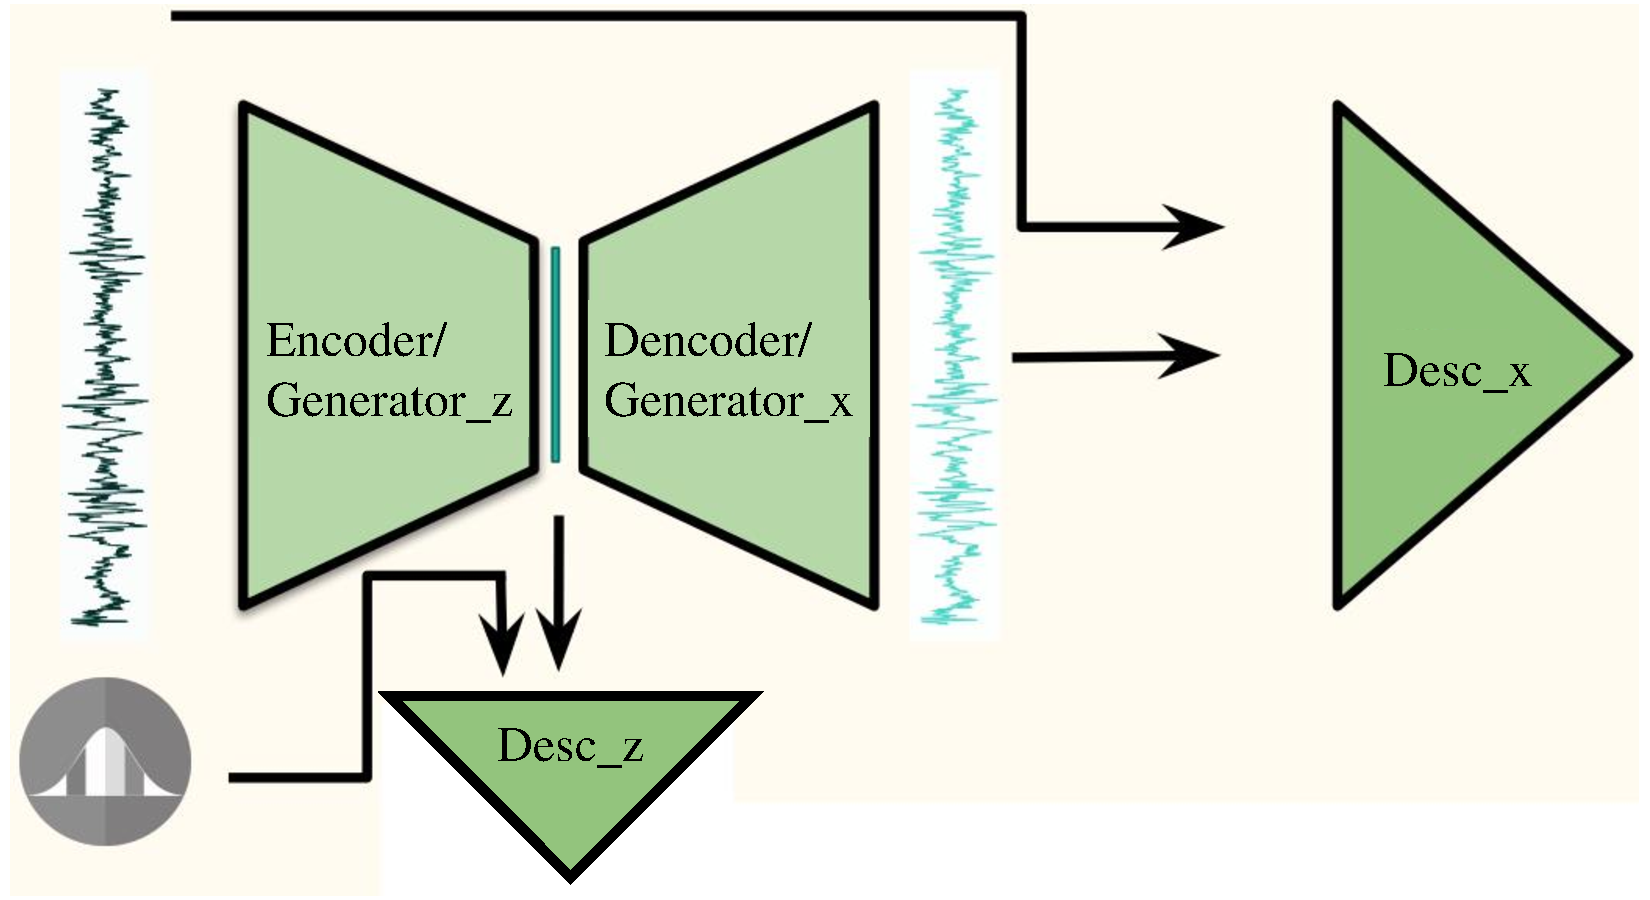
\includegraphics[width=0.9\linewidth]{figures/network_structure.pdf}
		\caption{Proposed network structure.}
		\label{workflow}
	\end{figure}
	\label{model}
	
	
	\section{Method}
	In this section, we describe the proposed adversarial autoencoder-based anomaly detection method in detail. The main idea is to train the model with only normal data and measure the deviation of test data from the learned distribution with two performance metrics: reconstruction error and distribution distance of latent vectors. Note that here we denote normal data is the data that belong to the period before disease induction procedure, which has nothing to do with mathematical normal distribution.
	
	\subsection{Proposed Model - Amr}
	We formulate our task as an unsupervised anomaly detection problem by learning only the distribution of the baseline EEG data through an adverserial autoencoder (AAE). AAE is formed of three sub-networks: encoder, decoder, and discriminator (see Fig. \ref{workflow}). The encoder is trained to map the input data into a lower-dimensional latent space $P(z|X)$, which the decoder uses to reconstruct the input $p(X|z)$. By being trained to discriminate between true samples from the prior distribution and the fake samples generated by the encoder, the discriminator generates a teaching signal to the encoder to generate latent space code that lies within the prior distribution. Specifically the discriminator is trained with the loss function:
	\begin{equation}
	\mathcal{L}_{D i s}=-\log (\operatorname{Dis}(\mathbf{z}))-\log (1-\operatorname{Dis}(\operatorname{Enc}(\mathbf{X})))
	\end{equation}
	where $z$ are the true samples from the prior distribution and $X$ are the data samples. On the other hand, the encoder and the decoder are trained with the loss function:
	\begin{equation}
	\mathcal{L}_{AE}= \left\Vert \mathbf{X} - \operatorname{Dec}(\operatorname{Enc}(\mathbf{X})) \right\Vert^2 -\log (\operatorname{Dis}(\operatorname{Enc}(\mathbf{X})))
	\end{equation}
	
	After training, the AAE can be used to scan the query data to look for deviations from the training data distribution. In the data space, anomalous data are expected to have high reconstruction errors and in the latent space, we hypothesize that they will deviate away from the center of the prior distribution used for training.
	Input data are 1 second EEG segments collected as described in section \ref{dataset} and sampled at 512 Hz. The encoder model is a simple 5 layer convolutional neural network with kernel size = 5, stride = 2 to consequently downsample the signal, and $2^{(3+k)}$ feature maps per layer $k$. Additionally, we added a final fully connected layer to flexibly map the features of the last convolutional layer to the desired dimension of the latent space, which in our case is 16. The decoder model reconstructs the input from the latent code through a fully connected layer and series of 5 transpose convolutional layers that sequentially upsample the signal and lower the number of feature maps till we reach the 512-dimensional input size.   
	
	\subsection{Cross-validation scheme}
	\textbf{I already mentioned it in the data set section.}
	yes, i have seen that, but this is confusing for me, because  I think the data set section should only be descriptive of the data, its collection and its preprocessing. I think the model should be described in details before we talk about its training! 
	We adopt leave-one-out (LOO) cross validation scheme where we iterate down the list of all rats (seven PPS rats and three control rats) we have and each trial we withhold the data from the rat completely. To be specific, during training, from the PPS group, we only use the data from the BL period, since the model is expected to capture the features in the BL period, such that it could detect signals that do not conform to the learned regularity, which is defined as anomaly. 
	To make sure that the model is learning EPG-related features and not the artifacts induced by the long-term recording, we use the data from the control rats, covering weeks of recordings time.   
	From the control group, we use the data spanning the whole recording period for training. The discrepancy of time period selections between the PPS group and the control group is due to the fact that it is common in longitudinal recordings, the long-term electrode implantation could cause an increased impedance of the electrode, which causes an increased high frequency component in the EEG signals \cite{straka2018characterizing}. During testing, we take the pre-trained model and scanning over all rat we have from the withheld rat.
	% i think the cross validation scheme should be in the experiment part not in the dataset part.
	
	To be specific, 1) we randomly selected 20 hours from each PPS animal from the BL period. 2) We randomly select 100 hours from the whole recording period from control animals. 3) we take non-overlapping one second EEG data as input to the model.
	
	
	
	\subsection{The testing process}
	After training the full model on the baseline data from 9 out of 10 animals, we tested the ability of the trained model to distinguish between baseline and epileptogenesis periods of the data from the withheld animal using two metrics: reconstruction error ($\mathcal{RE}$) and the distance of the latent code to the origin of the prior distribution ($\mathcal{D}$). 
	
	\begin{equation}
	\mathcal{RE(\mathbf{x})}= \left\Vert \mathbf{x} - \operatorname{Dec}(\operatorname{Enc}(\mathbf{x})) \right\Vert^2 
	\end{equation}
	
	\begin{equation}
	\mathcal{D}(\mathbf{x})= \left\Vert 0 - \operatorname{Enc}(\mathbf{x}) \right\Vert^2
	\end{equation}
	We set a threshold for these metrics based on the statistics of the training data e.g. $99^{th}$ percentile of the distribution of these metrics computed from the training dataset. In order to aggregate the evidence from longer recording time periods, and in the same time simulate a clinical setting, we compute the average number of surpathreshold segments within a certain time window e.g. 1 hour for both BL and EPG data of the test animal. Consequently, we evaluate the ability of this aggregated metric to distinguish between BL and EPG data by drawing the receiver operating characteristic (ROC) curve, and computing the area under the curve (AUC). We apply this process for the $\mathcal{RE}$ and $\mathcal{D}$ metrics. Moreover, we investigate our hypothesis that a weighted average of both metrics would lead to better classification results. The intuition behind the hypothesis is that anomalous features arising from the epileptogenesis process could be either local (affecting few timepoints), or global (affecting all timepoints of the training segments), and therefore would behave differently in the latent space and in the reconstructed data space.
	
	
	% \begin{equation}
	% \mathcal{D}(\mathbf{p}, \mathbf{z})=\sqrt{\sum_{i=1}^{n}\left(z_{i}-p_{i}\right)^{2}}
	% \end{equation}
	
	\subsection{Implementations and training settings}
	
	
	
	
	
	
	
	
	% 	The model is trained to learn a good compressed representation of the input data $Z$while retaining the 
	
	% 	There three components in our proposed framework: an autoencoder, trained with $\left\Vert x - \hat{x} \right\Vert^2$ that is able to extract the common features of variation from BL recordings and reconstruct them faithfully
	
	
	% 	There are two sources of anomaly: samples that are poorly reconstructed, i.e., with high reconstruction; the distance between the encoded latent representation distribution to the learned prior.
	% 	\subsection{Architecture}
	% 	We implemented an adversarial autoencoder for the unsupervised anomaly detection task.
	% 	\cite{makhzani2015adversarial}, 
	% 	\cite{yer2019detection} - detection of accounting anomalies in the latent space using adversarial autoencoder neural networks: 
	% 	\subsection{Naive classifier}
	%     \begin{itemize}
	%         \item what is the anomaly score for classification
	%     \end{itemize}
	% 	Put histogram as input to a classifier.
	
	% 	reconstruction error,
	
	% 	distance of current encoded latent vectors to the center of BL distribution
	% 	After the network has been trained on only BL data, we scan all the data from the withheld data
	
	
	
	\section{Experiment - Amr-Diyuan}
	
	\begin{itemize}
		\item plots: error evolution in one example animal
		\item plot: histogram evolution in one example animal? potentially we could also use the error histogram to so a simple classification.
		\item plot2: error histogram for BL and EPG
		\item table: ROC performance with different metrics
		\item experiment on another data set? We could add the dataset from Massimo, where they also have BL
	\end{itemize}
	
	Explanation for sometimes the model have even lower loss in testing data than that in validation data could be linked to the fact that likelihoods from the generative models show a strong bias towards the complexity of the input data \cite{serra2019input, schirrmeister2020understanding, ren2019likelihood}. That is to say the generative model tends to generate lowest likelihoods for qualitatively complex signals, and relatively high likelihoods for simple signals.
	
	
	\subsection{Ablation Study}
	\begin{itemize}
		\item without control rats
		\item change the weights for ae loss weight, reg loss, gen z loss, gen x loss, dc loss? Have enough time? What is the most obvious and promising direction?
		\item visualize the features that have anomalous reconstruction error or latent vector.
	\end{itemize}
	
	
	To further understand different aspects of the proposed method, we perform ablation studies. Specifically, we aim to investigate the effectiveness of different loss components to the final EPG detection task. In this section, we perform ablation studies on components of our proposed network such that we could further understand what exactly are the features that are evolving in EPG that lead the brain to being epileptic.
	\begin{itemize}
		\item with only reconstruction error
		\item with only latent z
		\item with supra-threshold events and reconstruction errors
	\end{itemize}
	
	\section{Conclusion}
	
	
	
	\bibliography{icml2021}
	\bibliographystyle{icml2021}
	
	
	
	
\end{document}


% This document was modified from the file originally made available by
% Pat Langley and Andrea Danyluk for ICML-2K. This version was created
% by Iain Murray in 2018, and modified by Alexandre Bouchard in
% 2019 and 2021. Previous contributors include Dan Roy, Lise Getoor and Tobias
% Scheffer, which was slightly modified from the 2010 version by
% Thorsten Joachims & Johannes Fuernkranz, slightly modified from the
% 2009 version by Kiri Wagstaff and Sam Roweis's 2008 version, which is
% slightly modified from Prasad Tadepalli's 2007 version which is a
% lightly changed version of the previous year's version by Andrew
% Moore, which was in turn edited from those of Kristian Kersting and
% Codrina Lauth. Alex Smola contributed to the algorithmic style files.



% \subsection{Citations and References}

% Please use APA reference format regardless of your formatter
% or word processor. If you rely on the \LaTeX\/ bibliographic
% facility, use \texttt{natbib.sty} and \texttt{icml2021.bst}
% included in the style-file package to obtain this format.

% Citations within the text should include the authors' last names and
% year. If the authors' names are included in the sentence, place only
% the year in parentheses, for example when referencing Arthur Samuel's
% pioneering work \yrcite{Samuel59}. Otherwise place the entire
% reference in parentheses with the authors and year separated by a
% comma \cite{Samuel59}. List multiple references separated by
% semicolons \cite{kearns89,Samuel59,mitchell80}. Use the `et~al.'
% construct only for citations with three or more authors or after
% listing all authors to a publication in an earlier reference \cite{MachineLearningI}.

% Authors should cite their own work in the third person
% in the initial version of their paper submitted for blind review.
% Please refer to Section~\ref{author info} for detailed instructions on how to
% cite your own papers.

% Use an unnumbered first-level section heading for the references, and use a
% hanging indent style, with the first line of the reference flush against the
% left margin and subsequent lines indented by 10 points. The references at the
% end of this document give examples for journal articles \cite{Samuel59},
% conference publications \cite{langley00}, book chapters \cite{Newell81}, books
% \cite{DudaHart2nd}, edited volumes \cite{MachineLearningI}, technical reports
% \cite{mitchell80}, and dissertations \cite{kearns89}.

% Alphabetize references by the surnames of the first authors, with
% single author entries preceding multiple author entries. Order
% references for the same authors by year of publication, with the
% earliest first. Make sure that each reference includes all relevant
% information (e.g., page numbers).

% Please put some effort into making references complete, presentable, and
% consistent. If using bibtex, please protect capital letters of names and
% abbreviations in titles, for example, use \{B\}ayesian or \{L\}ipschitz
% in your .bib file.

% \section*{Software and Data}

% If a paper is accepted, we strongly encourage the publication of software and data with the
% camera-ready version of the paper whenever appropriate. This can be
% done by including a URL in the camera-ready copy. However, \textbf{do not}
% include URLs that reveal your institution or identity in your
% submission for review. Instead, provide an anonymous URL or upload
% the material as ``Supplementary Material'' into the CMT reviewing
% system. Note that reviewers are not required to look at this material
% when writing their review.

% % Acknowledgements should only appear in the accepted version.
% \section*{Acknowledgements}

% \textbf{Do not} include acknowledgements in the initial version of
% the paper submitted for blind review.

% If a paper is accepted, the final camera-ready version can (and
% probably should) include acknowledgements. In this case, please
% place such acknowledgements in an unnumbered section at the
% end of the paper. Typically, this will include thanks to reviewers
% who gave useful comments, to colleagues who contributed to the ideas,
% and to funding agencies and corporate sponsors that provided financial
% support.

% \section{Figures}
% \begin{figure}[ht]
% \vskip 0.2in
% \begin{center}
% \centerline{\includegraphics[width=\columnwidth]{icml_numpapers}}
% \caption{Historical locations and number of accepted papers for International
% Machine Learning Conferences (ICML 1993 -- ICML 2008) and International
% Workshops on Machine Learning (ML 1988 -- ML 1992). At the time this figure was
% produced, the number of accepted papers for ICML 2008 was unknown and instead
% estimated.}
% \label{icml-historical}
% \end{center}
% \vskip -0.2in
% \end{figure}


% \subsection{Algorithms}

% If you are using \LaTeX, please use the ``algorithm'' and ``algorithmic''
% environments to format pseudocode. These require
% the corresponding stylefiles, algorithm.sty and
% algorithmic.sty, which are supplied with this package.
% Algorithm~\ref{alg:example} shows an example.

% \begin{algorithm}[tb]
%   \caption{Bubble Sort}
%   \label{alg:example}
% \begin{algorithmic}
%   \STATE {\bfseries Input:} data $x_i$, size $m$
%   \REPEAT
%   \STATE Initialize $noChange = true$.
%   \FOR{$i=1$ {\bfseries to} $m-1$}
%   \IF{$x_i > x_{i+1}$}
%   \STATE Swap $x_i$ and $x_{i+1}$
%   \STATE $noChange = false$
%   \ENDIF
%   \ENDFOR
%   \UNTIL{$noChange$ is $true$}
% \end{algorithmic}
% \end{algorithm}


% \begin{table}[t]
% \caption{Classification accuracies for naive Bayes and flexible
% Bayes on various data sets.}
% \label{sample-table}
% \vskip 0.15in
% \begin{center}
% \begin{small}
% \begin{sc}
% \begin{tabular}{lcccr}
% \toprule
% Data set & Naive & Flexible & Better? \\
% \midrule
% Breast    & 95.9$\pm$ 0.2& 96.7$\pm$ 0.2& $\surd$ \\
% Cleveland & 83.3$\pm$ 0.6& 80.0$\pm$ 0.6& $\times$\\
% Glass2    & 61.9$\pm$ 1.4& 83.8$\pm$ 0.7& $\surd$ \\
% Credit    & 74.8$\pm$ 0.5& 78.3$\pm$ 0.6&         \\
% Horse     & 73.3$\pm$ 0.9& 69.7$\pm$ 1.0& $\times$\\
% Meta      & 67.1$\pm$ 0.6& 76.5$\pm$ 0.5& $\surd$ \\
% Pima      & 75.1$\pm$ 0.6& 73.9$\pm$ 0.5&         \\
% Vehicle   & 44.9$\pm$ 0.6& 61.5$\pm$ 0.4& $\surd$ \\
% \bottomrule
% \end{tabular}
% \end{sc}
% \end{small}
% \end{center}
% \vskip -0.1in
% \end{table}

% \section{Introduction}
% The guidelines below will be enforced for initial submissions and
% camera-ready copies. Here is a brief summary:
% \begin{itemize}
% \item Submissions must be in PDF\@.
% \item Submitted papers can be up to eight pages long, not including references, plus unlimited space for references. Accepted papers can be up to nine pages long, not including references, to allow authors to address reviewer comments. Any paper exceeding this length will automatically be rejected. 
% \item \textbf{Do not include author information or acknowledgements} in your
%     initial submission.
% \item Your paper should be in \textbf{10 point Times font}.
% \item Make sure your PDF file only uses Type-1 fonts.
% \item Place figure captions \emph{under} the figure (and omit titles from inside
%     the graphic file itself). Place table captions \emph{over} the table.
% \item References must include page numbers whenever possible and be as complete
%     as possible. Place multiple citations in chronological order.
% \item Do not alter the style template; in particular, do not compress the paper
%     format by reducing the vertical spaces.
% \item Keep your abstract brief and self-contained, one paragraph and roughly
%     4--6 sentences. Gross violations will require correction at the
%     camera-ready phase. The title should have content words capitalized.
% \end{itemize}

% \subsection{Submitting Papers}
% The style file uses the \texttt{hyperref} package to make clickable links in documents. If this causes problems for you, add \texttt{nohyperref} as one of the options to the \texttt{icml2021} usepackage statement.


% Do not anonymize citations in the reference section. The only exception are manuscripts that are not yet published (e.g., under submission). If you choose to refer to such unpublished manuscripts \cite{anonymous}, anonymized copies have to be submitted as Supplementary Material via CMT\@. However, keep in mind that an ICML paper should be self contained and should contain sufficient detail for the reviewers to evaluate the work. In particular, reviewers are not required to look at the Supplementary Material when writing their review.
